%%%%%%%%%%%%%%%%%%%%%%%%%%%%%%%%%%%%%%%%%%%%%%%%%%%%%%%%%%%%%%%%%%%%%%%%%%%%%%%%%%%%%
%																					%
%	TRABAJO: Paper Mejoras en el procesador de Redes de Petri						%
%																					%
%		Titulo: 	Soft Core parametrizable con procesamiento de Redes de Petri	%
%																					%
%		Autores:	Julian Nonino													%
%					Carlos Renzo Pisetta											%
%					Orlando Micolini												%
%																					%
%	Seccion: CRECIMIENTO DEL IP CORE												%	
%	Archivo: crecimiento_ip_core.tex												%
%																					%
%%%%%%%%%%%%%%%%%%%%%%%%%%%%%%%%%%%%%%%%%%%%%%%%%%%%%%%%%%%%%%%%%%%%%%%%%%%%%%%%%%%%%

\section{Crecimiento del IP Core}
		Se analiz� el crecimiento del procesador en funci�n de los par�metros que posee. 
		Para esto se generaron procesadores de 8x8, 16x16 y 
		32x32 con capacidad de 7 bits por plaza y elementos de tiempo de 48 bits 
		y se graficaron los valores que se pueden observar en la Figura \ref{fig:resultados09}.
		
		\begin{figure}[h]
			\centering
			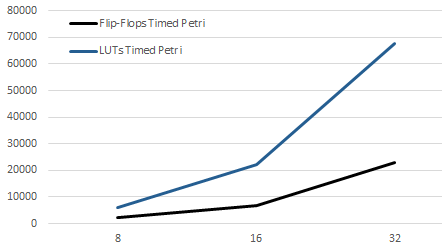
\includegraphics[width=3.5in]{./img/resultados09}
			\caption{Diferentes implementaciones del procesador de Redes de Petri}
			\label{fig:resultados09}
		\end{figure}

		Es observa que el crecimiento del IP Core no es algo para despreciar, puesto que 
		se incrementa r�pidamente a medida que aumentamos la cantidad de elementos soportados.
		Se observa tambi�n que si bien la pendiente aumenta, �stos incrementos son cada vez menores,
		tendiendo a linealizar para los IP Cores m�s grandes.

\section{Timed vs Time}

		Debido a la posibilidad de implementar Timed Petri Nets utilizando plazas y transiciones intermedias
		utilizando un procesador de Time Petries Nets, se compararon las curvas de crecimiento, las cuales se 
		muestran en la la Figura\ref{fig:timevstimed}
		
		\begin{figure}[h]
			\centering
			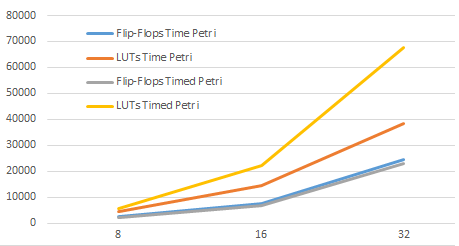
\includegraphics[width=3.5in]{./img/timevstimed} 
			\caption{Comparaci�n del crecimiento del IP Core}
			\label{fig:timevstimed} 
		\end{figure}

		Se Puede observar que el incremento de Flip-Flops se mantienen parejos, pero en el caso de las LUTs
		el crecimiento exponencial posee mayor pendiente en el Timed ip core, necesitando un 90\% mas que el
		Time ip core.  
		